\documentclass[10pt, twocolumn]{article}
\usepackage[top=.5in,left=.5in,right=.5in,bottom=1in]{geometry} 
\usepackage{amsmath,amsthm,amssymb,amsfonts}
\usepackage{enumitem} 
\usepackage{graphicx}
\graphicspath{ {../P2/} {../P3_ellen/} {../P4/}{../}}
\usepackage{listings}
\usepackage{color}
 
\usepackage[caption = false]{subfig}
\usepackage{sidecap}
\usepackage[normalem]{ulem}
\useunder{\uline}{\ul}{}
 
\definecolor{codegreen}{rgb}{0,0.6,0}
\definecolor{codegray}{rgb}{0.5,0.5,0.5}
\definecolor{codepurple}{rgb}{0.58,0,0.82}
\definecolor{backcolour}{rgb}{0.95,0.95,0.92}
 
\lstdefinestyle{mystyle}{
    backgroundcolor=\color{backcolour},   
    commentstyle=\color{codegreen},
    keywordstyle=\color{magenta},
    numberstyle=\tiny\color{codegray},
    stringstyle=\color{codepurple},
    basicstyle=\footnotesize,
    breakatwhitespace=false,         
    breaklines=true,                 
    captionpos=b,                    
    keepspaces=true,                 
    %numbers=left,                    
    numbersep=5pt,                  
    showspaces=false,                
    showstringspaces=false,
    showtabs=false,                  
    tabsize=2
}
 
\lstset{style=mystyle}
 
\newcommand{\N}{\mathbb{N}}
\newcommand{\Z}{\mathbb{Z}}
\newcommand{\C}{\mathcal{C}}
\newcommand{\D}{\mathcal{D}}
\newcommand{\R}{\mathbb{R}}
 
\begin{document}
 
\title{Techniques for linear regression}
\author{[redacted]}
\maketitle
 
In this paper we explore methods for regression of simple linear models. In section 1, we begin by discussing a popular method for the numerical optimization of differentiable cost functions: gradient descent. We compare two variants of its implementation, batch gradient descent (BGD) and stochastic gradient descent (SGD), and discuss their convergence characteristics. In section 2, we benchmark the performance of gradient descent on the least squares fitting of simple linear models on generated data and compare its performance against the analytic solution. Since the generated data is known The simplicity of the data allows us to study the effect of model selection as we consider both polynomial basis functions and cosine basis functions for the fitted model. Finally, in sections 3 and 4, we explore the effect of ridge and LASSO regularization, respectively, in model optimization and discuss their implications on the bias-variance tradeoff of the fitted parameters.

\section{Gradient Descent}

\subsection{Batch Gradient Descent on Gaussian and Quadratic Objective Functions}

We implemented a basic batch gradient descent procedure for minimizing functions and tested this procedure on a Gaussian and  a quadratic function (Figure \ref{fig:1.1}). These functions have known minima at (10,10) and ($26.67,26.67$) respectively. This procedure takes in a constant step size, a starting guess vector, and a criteria for convergence. We examined the effects of these parameters.
 
 \medskip

 \textbf{Step Size}: For both functions, decreasing the step size caused the gradient descent procedure to converge slower (Fig \ref{fig:1.1}a,e). This makes sense as a smaller step size will cause a smaller update in each iteration. 
 
  \textbf{Starting Guess}: The effect of the starting guess varied between the Gaussian and Quadratic functions (Fig \ref{fig:1.1}b,f). For the Gaussian function, whose minimum is at (10,10), the number of iterations to convergence increases as the Euclidean distance between the starting guess and true minimum increases. Furthermore since starting guesses (5,15) and (15,5) are the same distance from the minimum, they converge at exactly the same rate. On the other hand, the time to convergence of the quadratic function generally increases with the distance from the starting guess to the minimum, although not in all cases. Since the covariance of the two inputs is non-zero, the function produces different results for (16.67, 36.67) and (16.67, 16.67) which have the same Euclidean distance from the minimum at (26.67,26.67). When starting at (16.67,16.67) the function starts off higher but converges faster than when starting at (16.67,36.67). The convergence is slower at the second point because the covariation term will make it hard to increase the first variable while decreasing the second variable. 
  
\textbf{Convergence criteria}: For both functions there is an inverse relationship between the number of iterations to convergence and the $\log_{10}$ of the convergence criteria (Fig \ref{fig:1.1}c,g). This makes sense as decreasing the convergence criteria by a factor of 10 will mean that the gradient descent procedure must get closer to the true minimum before terminating

\medskip
Furthermore, for both functions we examined the norm of the gradient (Fig \ref{fig:1.1}d,h). In both cases, the norm of the gradient monotonically decreases and goes close to 0 at the time of convergence.

\begin{figure}[!h]

\subfloat[]{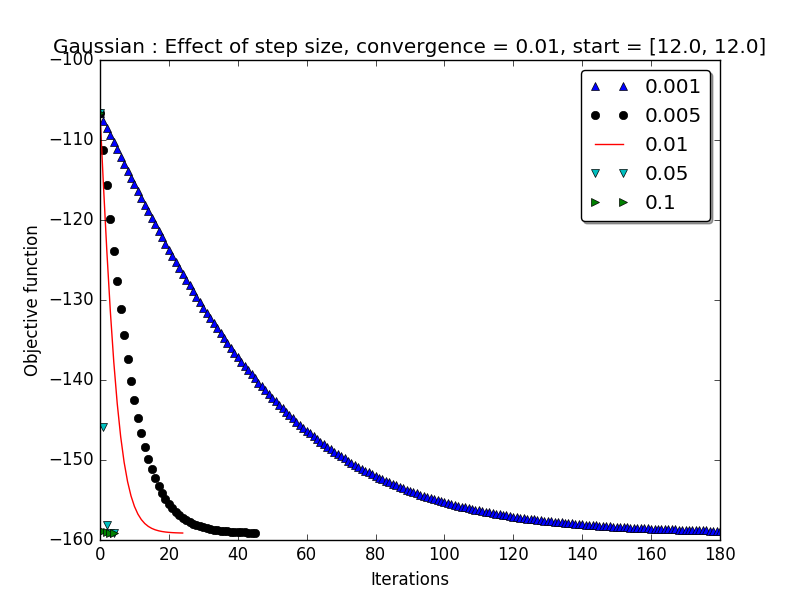
\includegraphics[width = 2in]{guassian_step_size.png}}
\subfloat[]{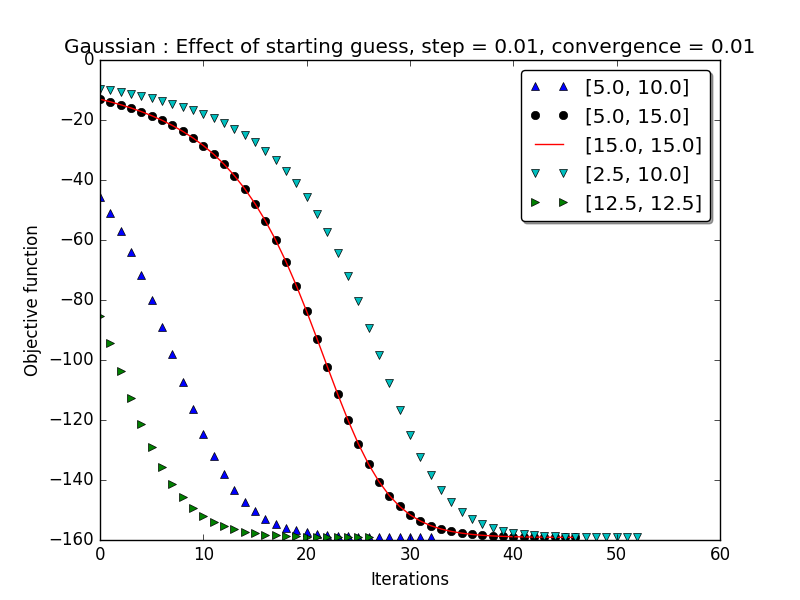
\includegraphics[width = 2in]{gaussian_starting.png}}
\subfloat[]{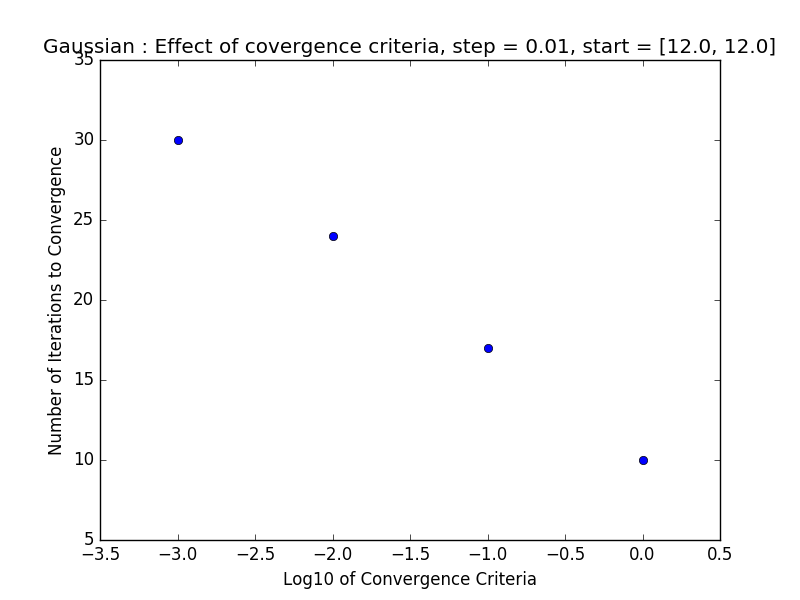
\includegraphics[width = 2in]{gaussian_convergence_criteria.png}}
\subfloat[]{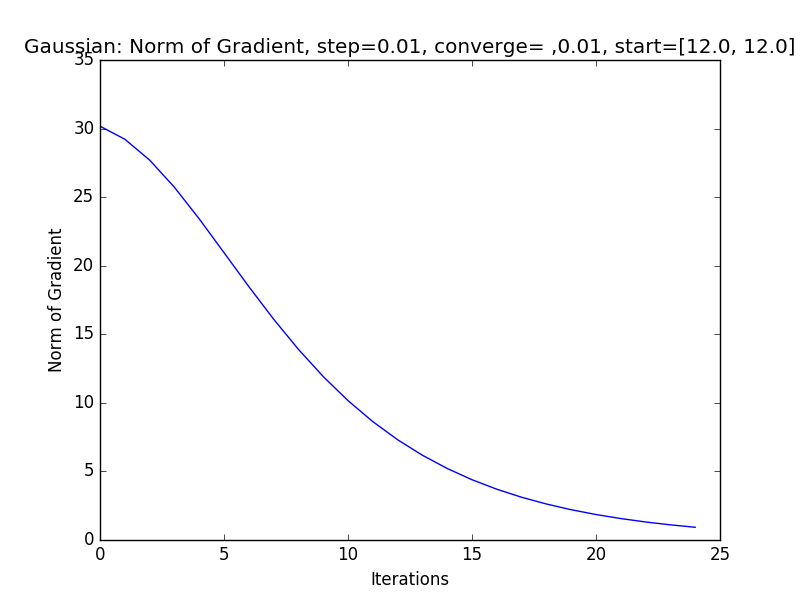
\includegraphics[width = 2in]{gaussian_gradient_norm.png}}
\\

\subfloat[]{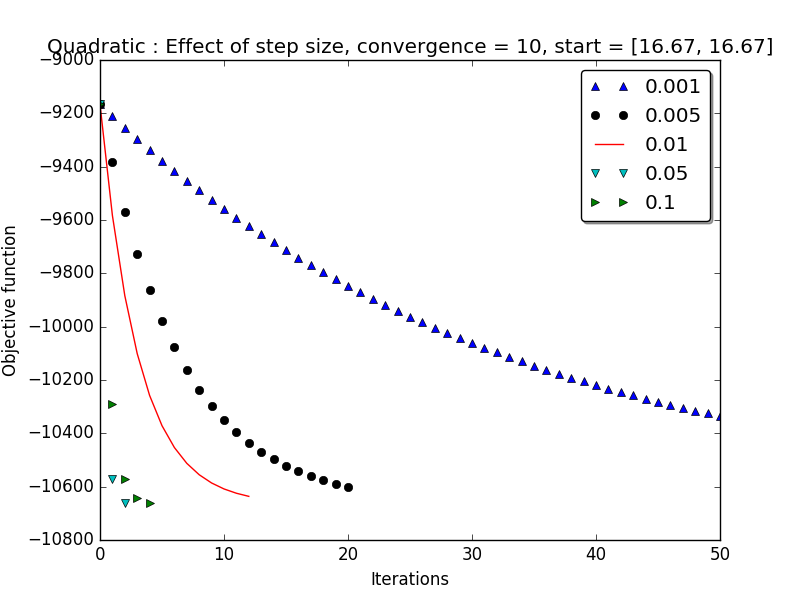
\includegraphics[width = 2in]{quadratic_step_size.png}}
\subfloat[]{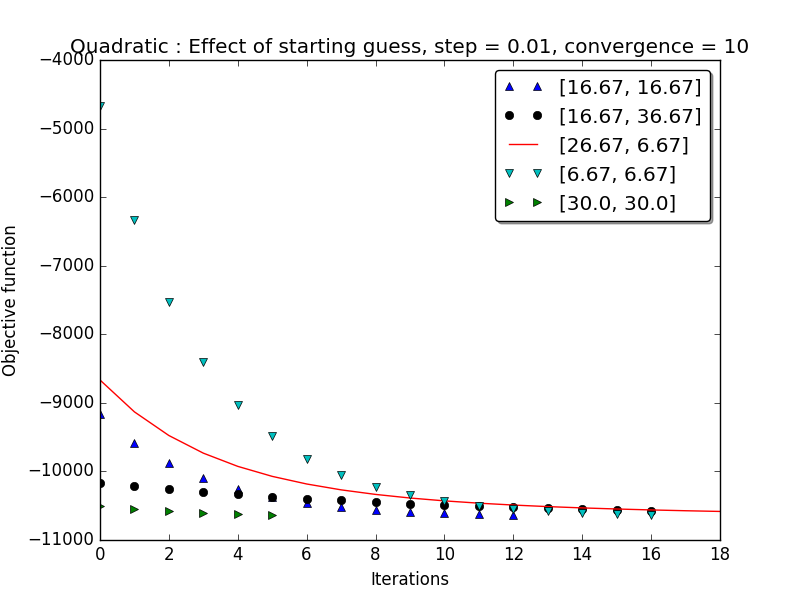
\includegraphics[width = 2in]{quadratic_starting.png}}
\subfloat[]{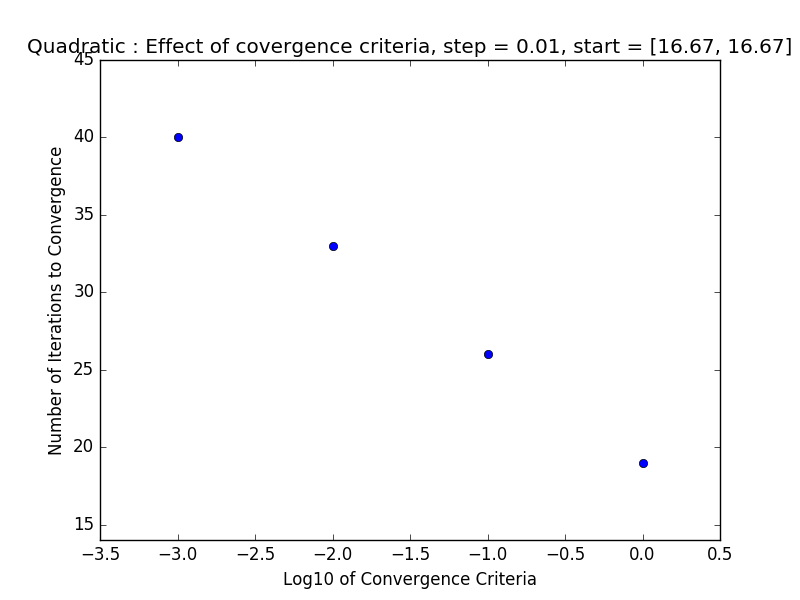
\includegraphics[width = 2in]{quadratic_convergence_criteria.png}}
\subfloat[]{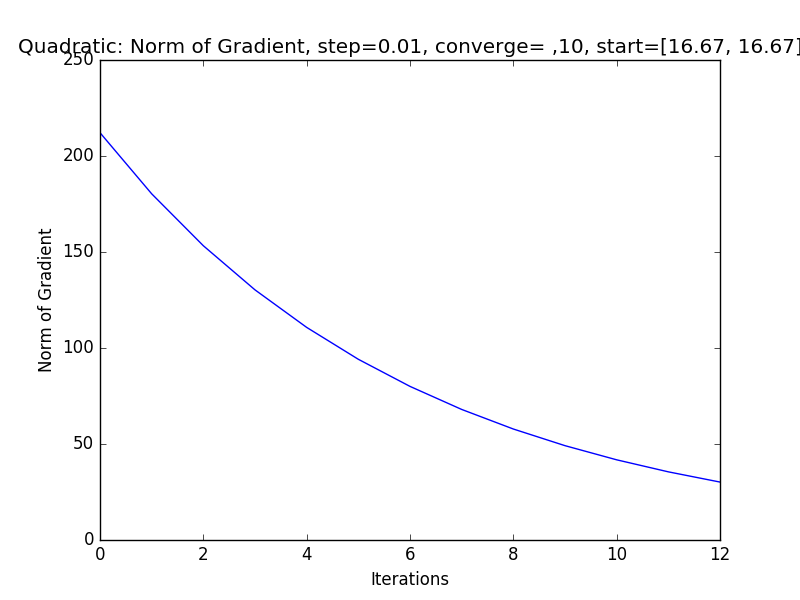
\includegraphics[width = 2in]{quadratic_gradient_norm.png}}
\caption{Batch gradient descent convergence characteristics on a gaussian and quadratic function. }
\label{fig:1.1}
\end{figure}

\begin{figure}[!h]
\centering
\subfloat[]{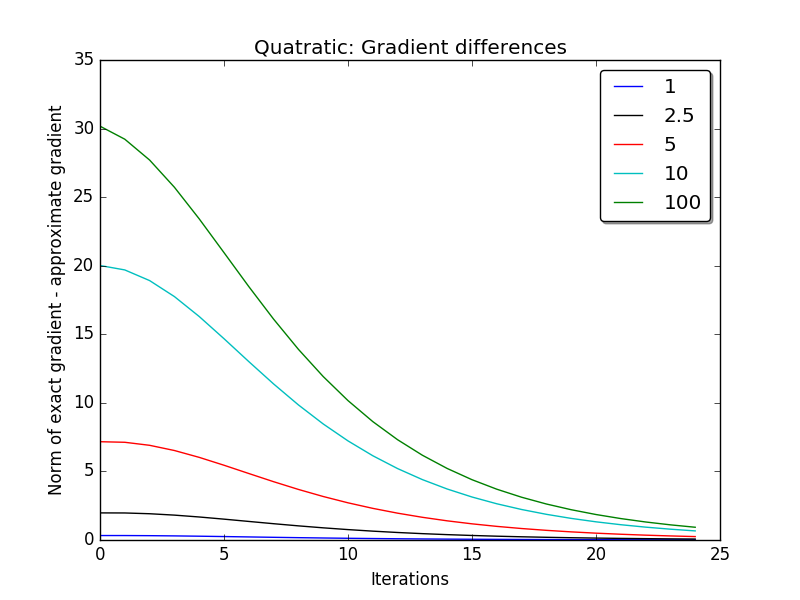
\includegraphics[width = 2in]{gaussian_finite_difference.png}}
\subfloat[]{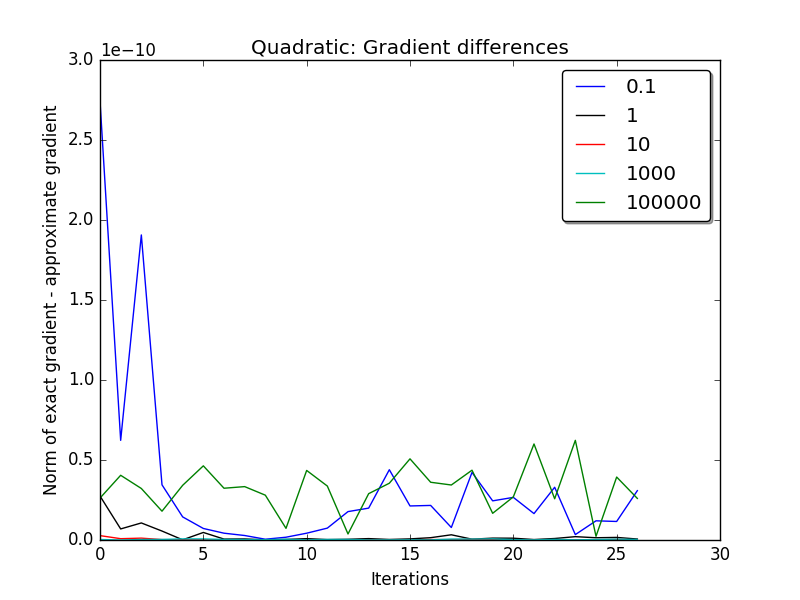
\includegraphics[width = 2in]{quadratic_finite_difference.png}}

\caption{The norm of the difference between the exact gradient and the central difference approximate gradient evaluated as the gradient descent procedure minimizes an objective function. Varied over different step sizes for the approximation. (A) Gaussian function with parameters from Fig 1d and (B) Quadratic function with parameters from Fig 1h}
\label{fig:1.2}
\end{figure}


\subsection{Central Difference Approximation}

 We used the central difference approximation to evaluate the value of the gradient during the course of a gradient descent procedure. Figure \ref{fig:1.2} displays the norm of the difference between the exact gradient and the approximate gradient over the course of gradient descent on the Gaussian and Quadratic functions. For the Gaussian function, the approximate gradient is much further from the exact gradient than is the case for the Quadratic function. This is because the secant line used by the central difference approximation is similar to the derivative of a quadratic function but is very different from the derivative of a Gaussian function. Note that the y-axis of Figure \ref{fig:1.2}a is on the scale of $10^1$ while the y-axis of Figure \ref{fig:1.2}b is on the scale of $10^{-10}$. Over this range of approximation step sizes, the Gaussian approximate gradient becomes more similar to the Gaussian gradient as the step sizes decreases. On the other hand, the Quadratic approximate gradient is most similar to the Quadratic exact gradient at a step size in the 1 to 10 range. At step sizes higher and lower the difference is greater. This is likely due to the fact that in the central difference approximation we move away from a point by the step size and divide the approximation by the step size. Thus too large of step size will move the approximation too far away, causing inaccuracy, while too small of a step size will produce a large value when the step size is divided, also creating inaccuracy. Thus there exists a sweet spot for the step size, where it is neither too large nor too small and produces the best results. 

\subsection{Stochastic Gradient Descent}

In addition to our batch gradient descent procedure, we implemented an alternative procedure using stochastic gradient descent. In this procedure, the learning rate at time $t$ is given by $\eta = (10^8 +t)^{-0.75}$. In Figure \ref{fig:1.3}, we compare batch and stochastic gradient descent when minimizing least squares data. For all starting points, stochastic gradient descent requires slightly more evaluations of the gradient than batch gradient descent does, although this difference is small relative to the total number of evaluations carried out. The similar number of iterations required by both methods is due to the fact that both of the objective functions are convex. If that was not true, we would expect stochastic gradient descent to work much better as it would more easily avoid local minima and saddle points when compared to batch gradient descent.

\medskip

Furthermore, batch gradient descent produces a weight vector whose relative distance from the ideal weight vector varies only slightly at the different start points. On the other hand, the relative distance of the weight vector with stochastic gradient descent varies much more so and is sometimes larger than that of batch gradient descent and sometimes smaller. This reflects the stochastic nature of stochastic gradient descent.

\begin{figure}
\centering
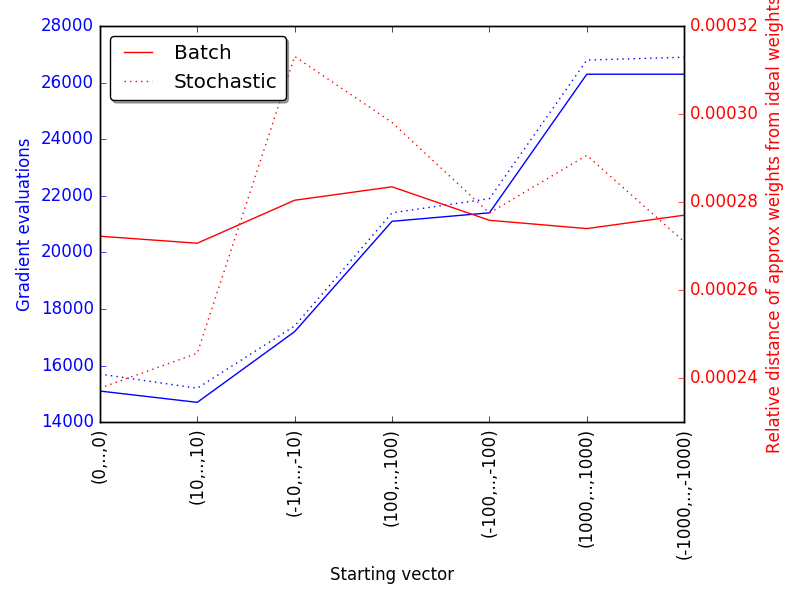
\includegraphics[width=.4\textwidth,height =0.25\textheight]{batch_stochastic_comp.png}
\caption{\label{fig:1.3}: Comparing batch and stochastic gradient descent for minimizing least squares objective. The number of gradient evaluations (blue) and the relative distance of the calculated weights from the ideal weights (red) for both batch gradient descent (solid line) and stochastic gradient descent (dotted line) at a variety of starting points.}
\end{figure}

\section{Linear Basis Function Regression}

Linear models are a popular choice of regression model due to their computational simplicity and interpretability. In a linear model, the model $f$ used to predict the observed data is expressed as a linear combination of terms:
$$ f(w,x) = \sum_i w_ig_i(x) $$
where $g$ are basis functions that transform the input data $x$, and $w$ are weights on each term. Note that while $g$ may involve a nonlinear transformation of $x$; the model is considered a linear model as long as it is linear in the parameters $w$. We can express $f$ in matrix form as
$$f(w,x) = \Phi w$$
where the ith column vector of $\Phi$ is $g_i(x)$. 

In the fitting of $n$ pairs of $(x,y)$ observational data, we first choose the functional form via selection of the basis functions $g_i$, and subsequently fit our model parameters $w_i$ by minimizing the sum of the square error (SSE) between the model prediction and the observed output: 
$$ argmin_w \theta(w) = argmin_w \sum_n (y_n - f(w,x_n))^2$$ % todo: define indexing variables
Alternative formulations of the problem exist where we simultaneously consider the space of potential models in the fitting process, however, that is outside the scope of this work.

The minimization of $\theta$ for linear basis functions has a closed form solution (Equation [below]). In the subsequent sections, we explore the tradeoffs between different choices of basis functions, and we use the analytically computed weights for various choices of linear basis function to benchmark gradient descent minimization of $\theta$ and gain intuition on its convergence properties. 

$$w = (\Phi^T\Phi)^{-1}\Phi^Ty$$

\subsection{Linear regression with a polynomial basis}

Eleven data points were generated under the following function with added noise:

$$f(x) = cos(\pi x) + cos(2\pi x); x \in [0,1]$$

Ignoring the true basis, we instead try to fit the data using a polynomial basis $\phi_0(x) = 1, \phi_1(x) = x, \phi_2(x) = x^2, ... , \phi_M(x) = x^M$, with GLS.  Figure \ref{fig:polyfit} shows fitted polynomials of variable order $M$ and highlights the tradeoff between model complexity and the quality of fit to the training data. At M=0 and M=1, the model is too simple and we have a large SSE. At the other extreme, with M=10, the model is able to exactly fit in the input data (SSE=0), including its noise. We see that at high values of M, our fitted polynomials oscillate between points and deviate from the true model even within the range of the training data. Furthermore, since we know the true model is a sum of cosines, the extrapolative power of any of these polynomial basis models outside the training range of $x \in [0,1]$ is poor, thus underscoring the danger of using a model to predict outside the range of its training data.

\begin{figure}
\caption{Input data and fitted models with polynomial basis functions. As the polynomial order M increases, the sum of square error (SSE) between the fitted polynomial and the input data decreases, however the risk of overfitting increases.}
\begin{center}
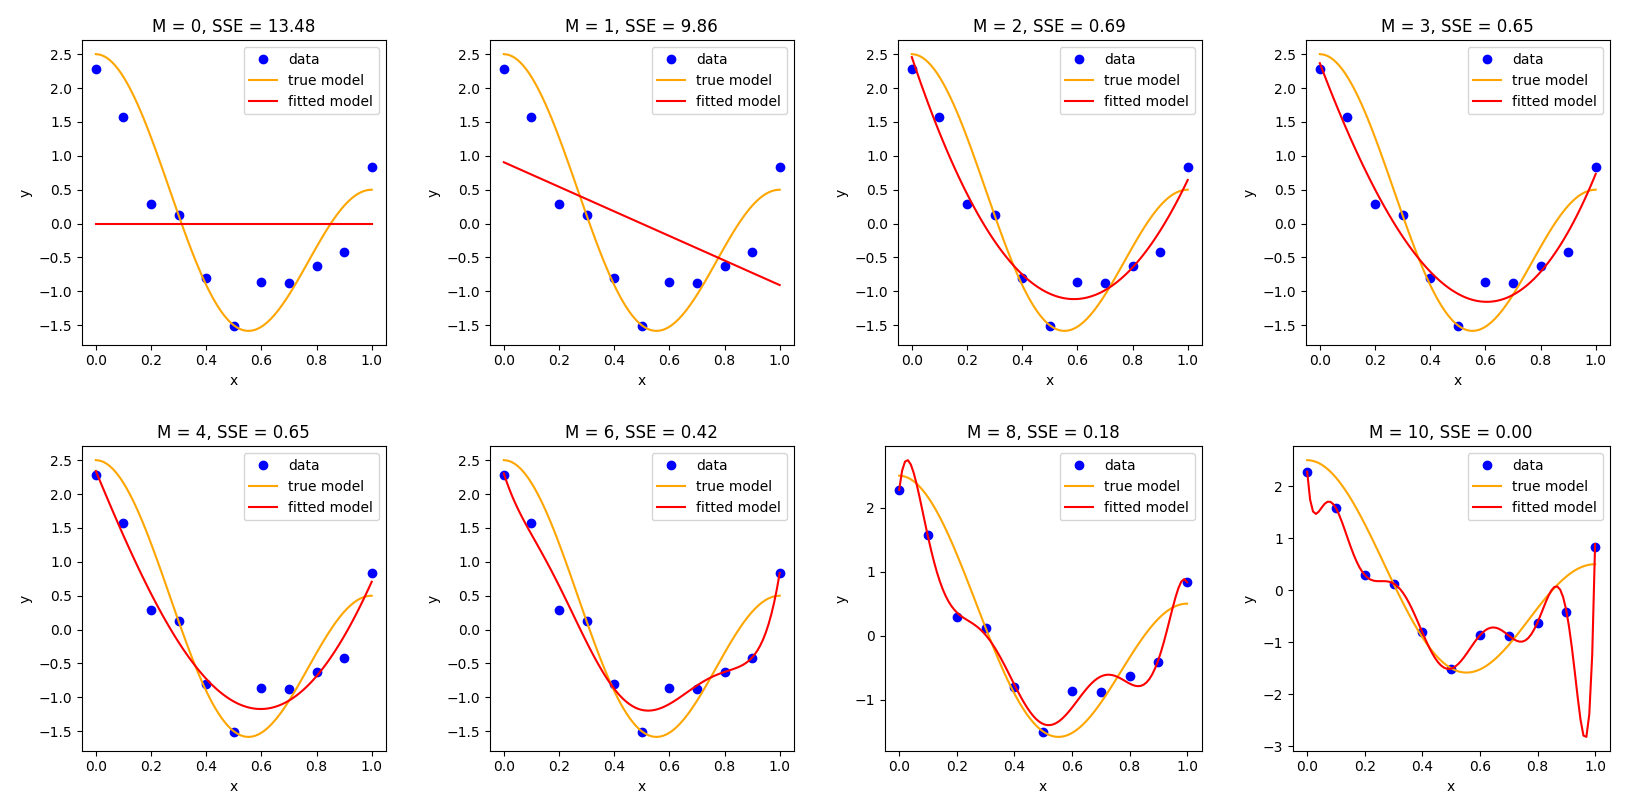
\includegraphics[width=200px]{all_regress_m}
\end{center}
\label{fig:polyfit}
\end{figure}

%\begin{table}
%\caption{Fitted weight vectors for linear regression of Equation [ref] with linear basis functions of increasing order.}
%\begin{center}
%\begin{tabular}{r | l}
%M=0 &  w =  [-0.001] \\
%M=1 &  w =  [0.906, -1.813] \\
%M=2 &  w =  [2.456, -12.15, 10.338] \\
%M=3 &  w =  [2.367, -10.731, 6.616, 2.481] \\
%M=4 &  w =  [2.341, -9.819, 2.055, 9.779, -3.649] \\
%M=6 &  w =  [2.304, -12.728, 63.938, -335.924, 783.22, -784.539, 284.565] \\
%M=8 &  w =  [2.278, 38.737, -972.518, 7401.42, -27960.868, 58014.38, -67074.038, 40504.018, -9952.576] \\
%M=10 &  w =  [2.278, -73.082, 2283.818, -30586.685, 208190.139, -813749.26, 1934260.6, -2841219.608, 2518054.828, -1233682.014, 256519.873] \\
%\end{tabular}
%\end{center}
%\label{poly_weights}
%\end{table}


\subsection{Performance of BGD and SGD}

Next we explore the performance of BGD and SGD on the same fitting problem with linear polynomial basis functions. We observe that both BGD and SGD have trouble reproducing the optimal values of $w$ for higher order polynomials (Figure \ref{fig:gd_weights}). 

\begin{figure}
\caption{Gradient descent methods have trouble reproducing the analytically computed optimal weights for higher order polynomials.}
\begin{center}
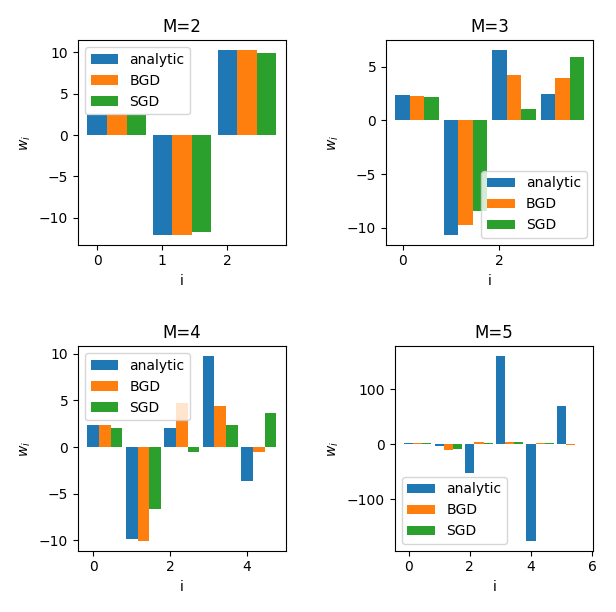
\includegraphics[width=200px]{all_weights}
\end{center}
\label{fig:gd_weights}
\end{figure}

This is a consequence of both having a model that is too complex for the given data and the stopping criterion in gradient descent methods; since there are a large number of higher order polynomials that can approximate our 11 data points, the SSE between any two of these functions will be small. Accordingly, we observed that changing the initial value changes the gradient descent solution for $w$. Additionally, if the convergence threshold is set to an extremely low value, the number of iterations goes up drastically since the difference in the objective between near-optimal solutions is very low. SGD is less susceptible to this problem since the algorithm is inherently noiser. Finally, since our underlying data was generated from a cosine basis, i.e. even functions, we note that increasing the order to an odd values usually leads to sharp increases in the number of iterations to convergence (Figure \ref{fig:iter_vs_M}).

\begin{figure}
\caption{As the polynomial order M increases, the number of iterations to convergence increases. The tolerance for both BGD and SGD was 1e-6. BGD used a step size of 0.01. SGD used a learning rate given by $k=0.75, \tau=100$.}
\begin{center}
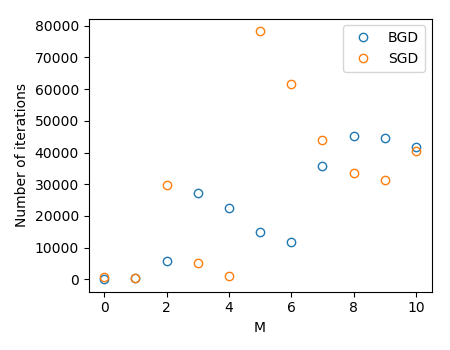
\includegraphics[width=200px]{iter_vs_M}
\end{center}
\label{fig:iter_vs_M}
\end{figure}

\subsection{Linear regression with a cosine basis}

Using a cosine basis of the form $\phi_1(x) = cos(\pi x), \phi_2(x) = cos(2\pi x), ... , phi_M(x) = cos(M\pi x)$, we fit the same data as in Section 2.1 (Figure \ref{fig:cos_fitting}). Since the cosine basis contains the true basis used to generate the data, we observe low SSE for $M>=2$ and a good qualitative match to the true model for intermediate values of M. At larger values of M, we start overfitting to the noise in the generated data. For example, at M=8, $w_{opt} =  (0.769, 1.087, 0.099, 0.143, -0.051, 0.362, 0.012, 0.015) $. While $w_1=0.77$ and $w_2=1.09$ are close to the true model $w_1 = w_2 = 1$, higher order terms have nonzero weight. In the next section, we discuss how regularization techniques may be used to enforce prior beliefs on our model parameters to avoid overfitting to noise.

\begin{figure}
\caption{As the cosine order M increases, the sum of square error (SSE) between the fitted model and the input data decreases, however the risk of overfitting increases.}
\begin{center}
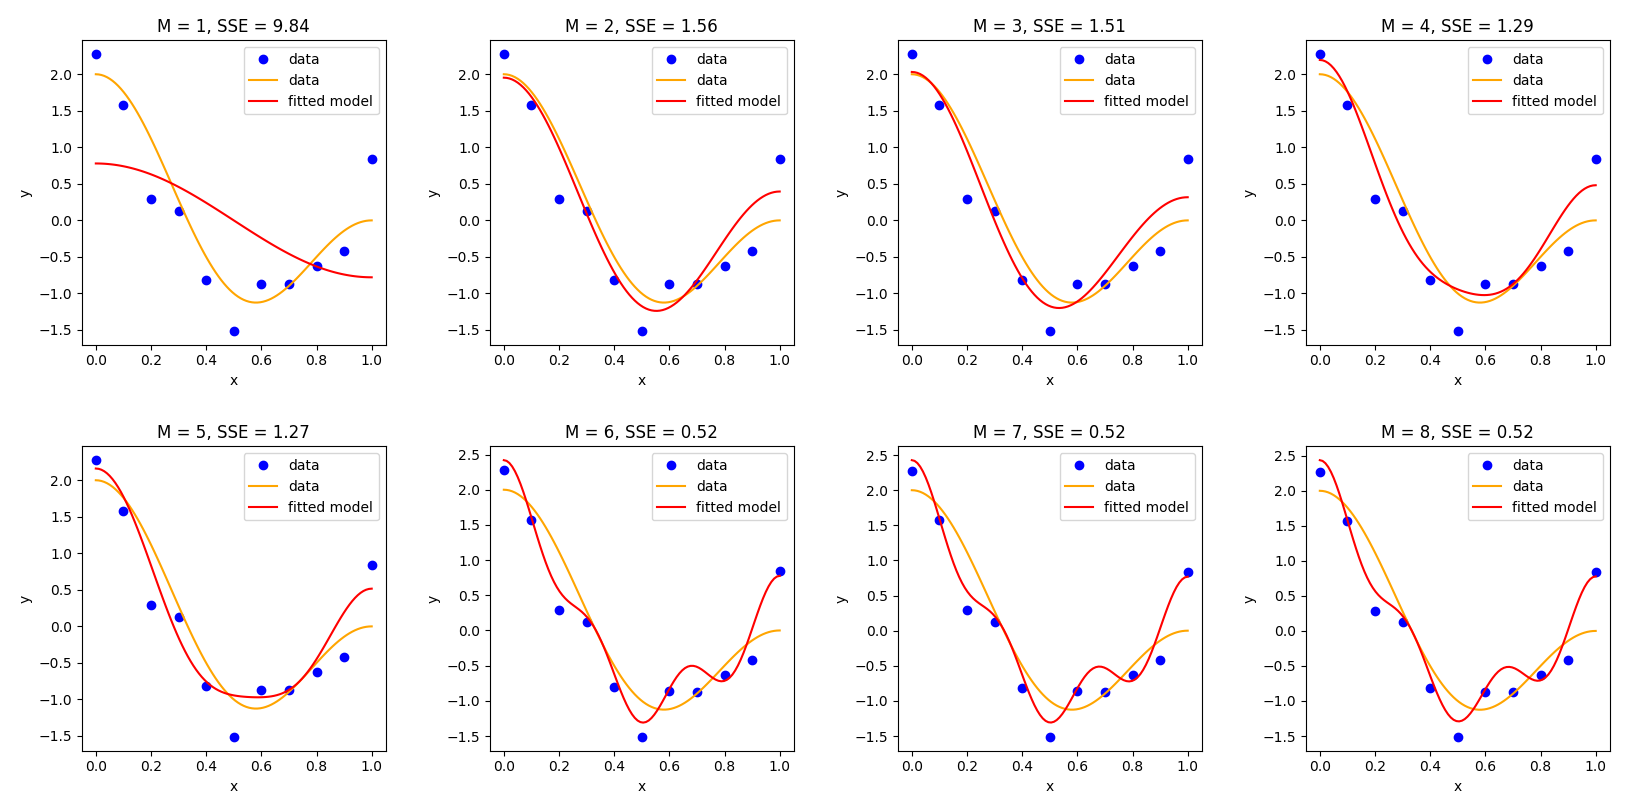
\includegraphics[width=200px]{all_regress_cos}
\end{center}
\label{fig:cos_fitting}
\end{figure}

%\begin{table}
%\caption{Fitted weight vectors for linear regression of Equation [ref] with cosine basis functions of increasing order.}
%\begin{center}
%\begin{tabular}{r | l}
%
%M=1 &  w =  [0.779] \\
%M=2 &  w =  [0.779, 1.174] \\
%M=3 &  w =  [0.763, 1.174, 0.094] \\
%M=4 &  w =  [0.763, 1.141, 0.094, 0.197] \\
%M=5 &  w =  [0.77, 1.141, 0.101, 0.197, -0.049] \\
%M=6 &  w =  [0.77, 1.089, 0.101, 0.145, -0.049, 0.363] \\
%M=7 &  w =  [0.769, 1.089, 0.099, 0.145, -0.051, 0.363, 0.012] \\
%M=8 &  w =  [0.769, 1.087, 0.099, 0.143, -0.051, 0.362, 0.012, 0.015] \\
%\end{tabular}
%\end{center}
%\label{cosine_weights}
%\end{table}

\section{Ridge Regression}

Ridge regression is a simple extension of generalized least squares which includes a second order regularization term to the error function. The relative importance of this regularization term is controlled by a parameter $\lambda$. 

$$f(w,x) = \Phi w + \lambda w^Tw$$

In a Baeysian framework, ridge regression represents including a prior that our weight parameters come from a gaussian distribution. In a frequentist framework, ridge regression is interpreted as adding a bias to our weight parameters in order to reduce the variance in our optimized weights. An advantage of regularization is that it allows model complexity to be tuned by adjusting the value of $\lambda$. In this section, we see how adding regularization affects our regressed parameters and how it allows us to fit a complex model to our data without severe overfitting.


We performed ridge regression with a polynomial basis on the same data set as in Section 2.1. We see that at M=8, using ridge regression dramatically reduces the magnitude of the fitted parameters and avoids overfitting. At sufficiently high values of lambda, we see our error function increase and the quality of fit decrease as our fitted function approaches a flat line.

% Figure: data fitted at M = 8 with different values of lambda
% Figure: total error, bias, variance vs lambda for different values of M

Next, we explore the optimization of our model parameters, $M$ and $\lambda$, on a data set split into set A, B, and a validation set (shown in Figure \ref{fig:P3_test}). We measured the performance of each training on A and testing on B and vice versa, with validation performed on the validation set.

\begin{figure}
\caption{Fitted weights using different values of $\lambda$}
\begin{center}
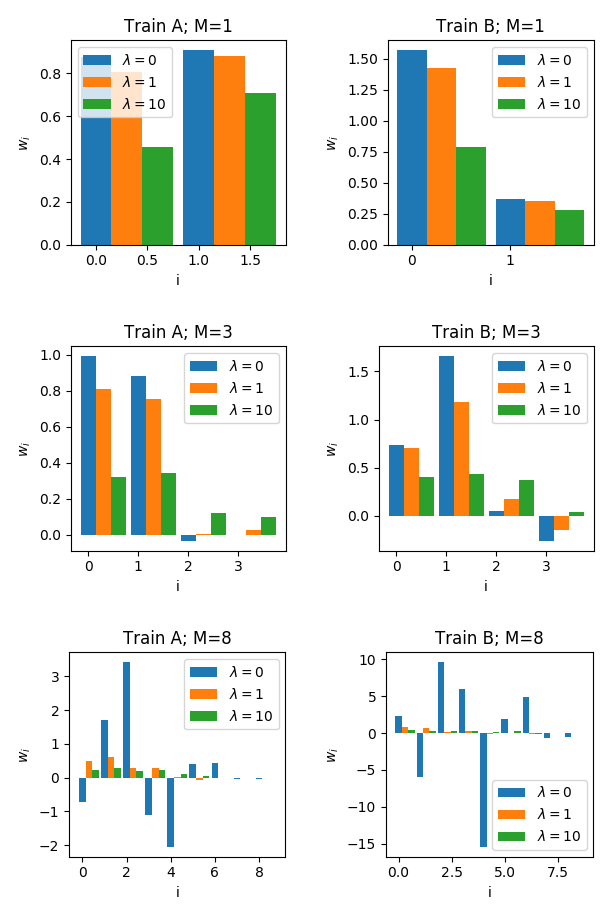
\includegraphics[width=200px]{P3_all_weights}
\end{center}
\label{fig:P3_all_weights}
\end{figure}

To help choose a model, we computed the Akaike information criterion (AIC) to assess the tradeoff between goodness of fit and model complexity (Figure \ref{fig:P3_AIC}). 

\begin{figure}
\caption{AIC is used to help select a model.}
\begin{center}
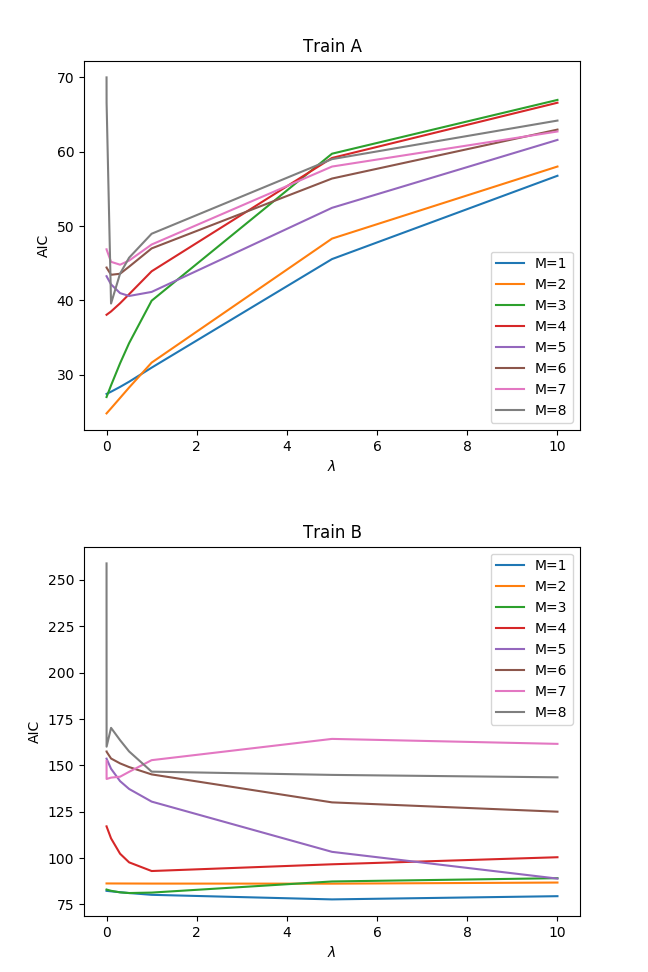
\includegraphics[width=200px]{P3_AIC}
\end{center}
\label{fig:P3_AIC}
\end{figure}

After training on dataset A (and ignoring dataset B), we selected $M=2$ and $\lambda=0$, the model that yielded the lowest AIC as computed with the validation dataset. After training on dataset B (and ignoring dataset A), we selected $M=1$ and $\lambda=5$. We then evaluated their performance on their test set (Figure \ref{fig:P3_test}). The model trained on A yields a SSE of 25.753 predicting the values from set B. The model trained on set B yields an SSE of 17.720 predicting the values of set A. Here, we observed a large variation between our fitted models due to an outlier in dataset B, which has an outsized effect from the small size of our data sets. An alternative procedure that may be better suited for a data poor regime is k-fold cross validation.

\begin{figure}
\caption{Testing our chosen model. The model trained on data A is specified by $M=2, \lambda=0$. The model trained on dataset B is specified by $M=1,\lambda=5$.}
\begin{center}
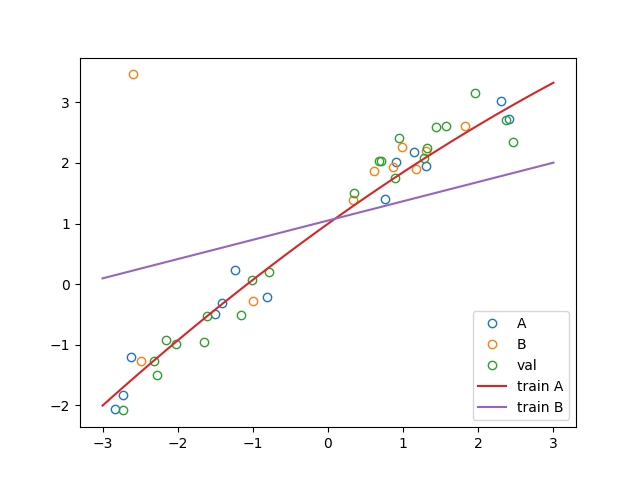
\includegraphics[width=200px]{P3_test}
\end{center}
\label{fig:P3_test}
\end{figure}

% training table for different values of M and lambda on training set: AIC, BIC, error
% validation table for different values of M and lambda on training set: AIC, BIC, error

% Figure: training error, testing error vs lambda... TODO

%We ran our ridge regression with a polynomial basis function on three datasets A, B and validation and tested the performance, as measured by $R^2$, in the following cases: training and regressing on A, training on A and regressing on B, training on A and regressing on validation, training and regressing on B, training on B and regressing on A, training on B and regressing on validation (Figure \ref{fig:3.2}). This was repeated for all parameter combinations of $M \in \{3,5,50\}$ and $\lambda \in \{0.1,10,100\}$. From the bottom two rows of the table, the highly negative $R^2$ values for $m=50$ make it clear than ridge regression heavily punishes model that severely overfit the data. Much better performance is seen with much more reasonable $M$ values such as 3 and 5. 

%\medskip

%However, it is also clear that there is danger in choosing a $\lambda$ value that is too high. From the top four rows of the table we can see that when $\lambda=10$ the model with $M=5$ outperforms the model with $M=3$ on the validation data. On the other hand, when $\lambda=100$ the model with $M=3$ is better than the one with $M=5$. However, this model is still performs worse on the validation set than both of the models generated with $\lambda = 10$. This illustrates that while increasing $\lambda$ is good for preventing overfitting, doing so runs the risk of generating a model with little predictive power.


\section{Sparsity and LASSO}

While the regularization in ridge regression penalizes high value parameters, LASSO regularization promotes sparsity by driving coefficients of certain basis functions to zero.

We trained, validated, and tested a dataset generated according to $y=w_{true}^T\phi(x) + \epsilon$, where $x,y \in \R, w \in \R^{13}$ and $\epsilon$ is a small noise. The feature vector is given by
$$ \phi(x) = (x, sin(0.4\pi x), sin(2*0.4\pi x),...,sin(12*0.4\pi x)) \in \R^{13}$$

\begin{figure}
\caption{Training LASSO and ridge regularization. Top panels show fitted models using different values of $\lambda$. Bottom panels show errors in the loss function and the AIC evaluated on the validation set.}
\begin{center}
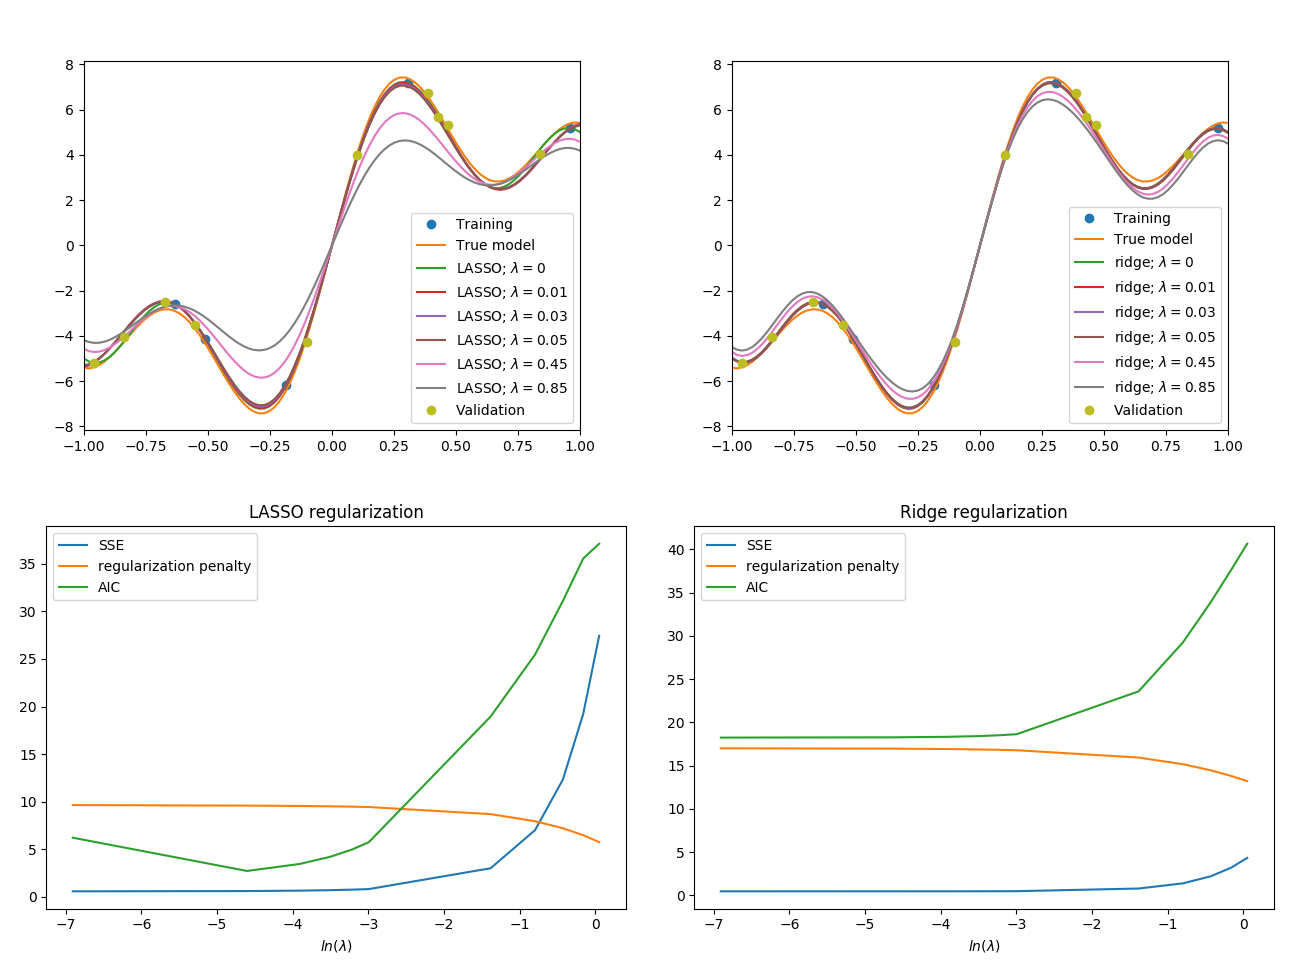
\includegraphics[width=270px]{all_training}
\end{center}
\label{fig:train_lasso}
\end{figure}

Our training results for various values of $\lambda$ for LASSO and ridge regularization are given in Figure \ref{fig:train_lasso}. After training each model, we use the validation data set to evaluate each set of parameters and choose an appropriate model. We see an inverse relationship between goodness of fit to the data and the regularization penalty. In order to compare different models, we compute the Akaike information criterion (AIC) to assess the tradeoff between goodness of fit and model complexity. Based on our computed AIC, we select the model with $\lambda=0.01$ for LASSO and $\lambda=0.01$ for ridge regression.

\begin{figure}
\caption{Fitting results.}
\begin{center}
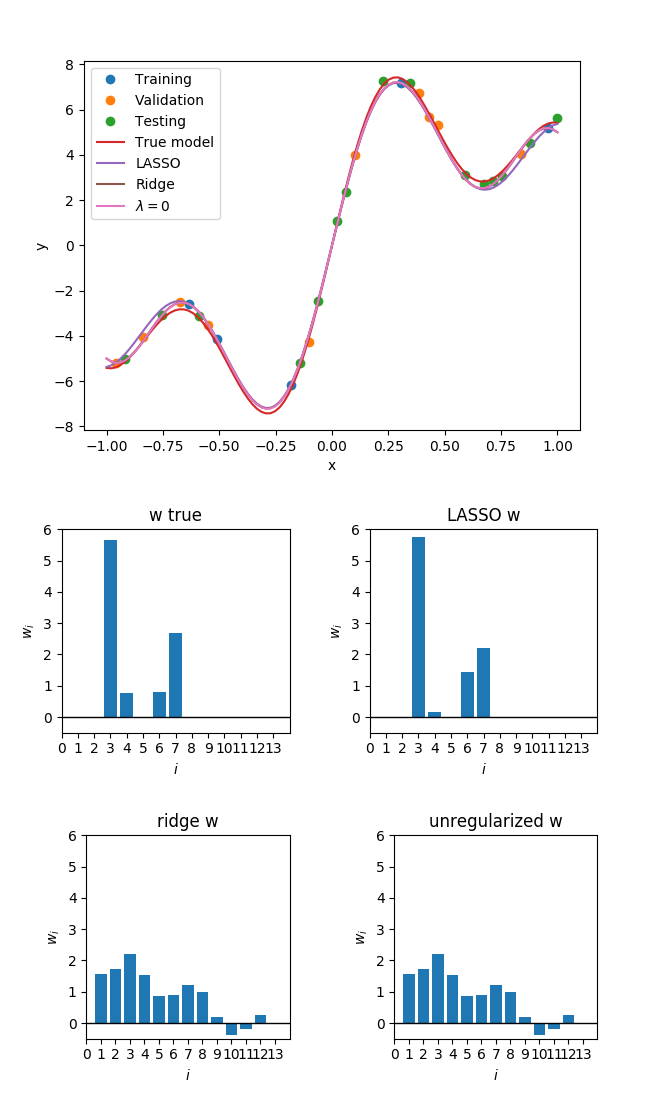
\includegraphics[width=200px]{final_fitting_results}
\end{center}
\label{fig:final_lasso_test}
\end{figure}

The optimized weights for each model is given in Figure \ref{fig:final_lasso_test}. While all models achieve a low error to the given data and qualitative agreement to the true model, visualizing the weights in the function shows that LASSO has most closely reproduced the true model. We also note that unregularized fitting yields parameters similar to ridge regression. This is likely a consequence of a small training set which only consists of 5 data points. We recommend combining the training and validation data sets used here and performing 3-fold cross validation for future work.

 %Finding the optimal LASSO weights has no closed form solution.

\section{Conclusions}

We have introduced batch gradient descent and stochastic gradient descent, two numerical methods used in the optimization of loss functions. We then introduced how gradient descent can be used in the context of generalized least squares and compared its performance for regression on linear models where there exists a closed form solution. We explore the relationship between the complexity of the model and the degree of overfitting in this data-poor context, thus motivating the introduction of regularization. We show how changing the regularization penalty tunes the model complexity, in particular, how ridge biases towards small parameter values and how LASSO biases towards sparse values.

 \end{document}